% \chapter{Analog machines from metamaterials}
\chapter{Metamaterial Mechanisms}
\label{chapter:analog-metamaterials}


% \section{Abstract}

% Recently, researchers started to engineer not only the outer shape of objects, but also their \textit{internal microstructure}. Such objects, typically based on 3D cell grids, are also known as metamaterials. Metamaterials have been used, for example, to create materials with soft and hard regions.

% So far, metamaterials were understood as materials---we want to think of them as \textit{machines}. We demonstrate metamaterial objects that perform a mechanical function. Such \textit{metamaterial mechanisms} consist of a single block of material the cells of which play together in a well-defined way in order to achieve macroscopic movement. Our metamaterial door latch, for example, transforms the rotary movement of its handle into a linear motion of the latch. Our metamaterial Jansen walker consists of a single block of cells---that can walk. The key element behind our metamaterial mechanisms is a specialized type of cell, the only ability of which is to shear. 

% In order to allow users to create metamaterial mechanisms efficiently we implemented a specialized 3D editor. It allows users to place different types of cells, including the shear cell, thereby allowing users to add mechanical functionality to their objects. To help users verify their designs during editing, our editor allows users to apply forces and simulates how the object deforms in response.


% \section{Introduction}

Researchers in HCI have explored the use of personal fabrication tools, such as 3D printers \cite{Tanenbaum2013} to help users design the external shape of 3D objects \cite{Weichel2014}. In order to add functionality to 3D printed objects, researchers integrated electronics \cite{Savage2013}, even printed optics \cite{Willis2012}, or loudspeakers \cite{Ishiguro2014}.

Researchers also started to design the inside of 3D objects by changing the structure of the 3D printed object itself. Initial projects optimized only a single parameter, such as the object’s strength-to-weight ratio \cite{Lu2014} or the position of the object’s center of mass \cite{Prevost2013}. 

Recently, researchers started to push internal structures even further and created objects that consist internally of large numbers of 3D cells organized on a regular grid \cite{Schumacher2015}. Since these objects allow each cell to be designed differently, the resulting objects literally offer thousands of degrees of freedom. These types of structures have also been referred to as \textit{metamaterials}. Metamaterials are artificial structures with mechanical properties that are defined by their usually repetitive cell patterns, rather than the material they are made of \cite{Paulose2015}. 

Based on this concept, researchers have created objects with unusual behaviors, such as metamaterials that collapse abruptly when compressed \cite{Mullin2007}, that shrink in two dimensions upon one-dimensional compression \cite{AlvarezElipe2012}, or objects that mix layers of soft and hard cells in order to emulate different materials \cite{Bickel2010a}. 

So far, metamaterials have been understood as materials. The main contribution of this paper is that we want to think of them as machines. 

In this work, we push the concept of metamaterials further by creating objects that allow for controlled directional movement. This allows users to create objects that perform mechanical functions. Our objects thereby implement devices that transform input forces and movement into a desired set of output forces and movement---also known as mechanisms. 


\section{Overview of metamaterial mechanisms}

Figure \ref{fig:1 metanism-door latch}a shows an example of a metamaterial mechanism: a door latch mechanism. Its interior is a regular grid of 3D cells; however, the cells are of different types. Figure \ref{fig:1 metanism-door latch}b shows how applying a force causes the cells to deform in a controlled way, thereby performing the intended mechanical function. In the example, rotating the door handle causes cells inside of the object to deform, ultimately pulling the latch towards the left and thereby unlocking the door.

\begin{figure}
    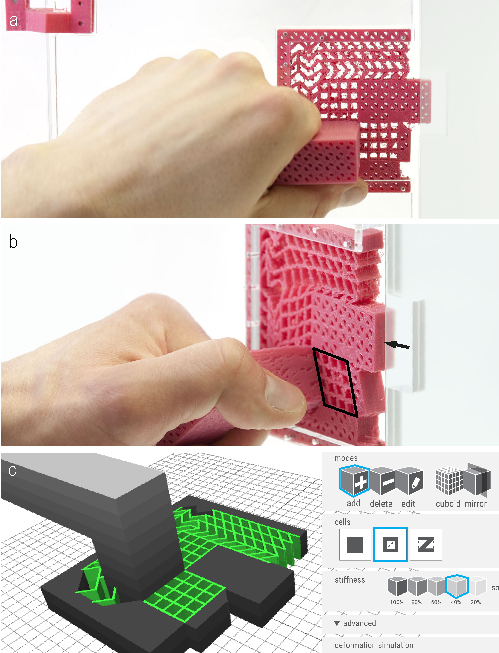
\includegraphics[width=\textwidth]{chapters/metamaterial-mechanisms-FIG/1-embedded-door-latch-figure1.pdf}
    \caption[Short figure name.]{(a) This door latch is implemented as a metamaterial mechanism; it consists of a single block of material based on a regular grid of cells that together implement handle, latch, and springs. (b) Turning the handle causes the central hinge array to deform and to pull the latch inwards, which unlocks the door. (c) We created this mechanism in our custom editor. Here, we placed two hinge arrays that mechanically couple the handle to the latch, and cells that couple to the doorframe.
    \label{fig:1 metanism-door latch}}
\end{figure}

While most of the object consists of \textit{rigid cells} (cells that are reinforced with a diagonal), the object also contains several rectangular regions of cells that lack such a diagonal reinforcement. These are the key to creating mechanisms, as they are able to deform in a very specific way: when subjected to an external force, these cells shear and thereby apply a force to their neighboring cells. We will discuss throughout the remainder of this paper how this basic principle allows creating mechanisms. 

Metamaterial mechanisms are simple. While the traditional door latch mechanism shown in Figure \ref{fig:2 metanism-traditional door latch} consists of several parts, including an axle, bearings, springs, etc., the metamaterial door latch in Figure \ref{fig:1 metanism-door latch} consists of a single block of material, as it is groups of cells inside the object that perform the mechanical function.

\begin{figure} [h]
    \includegraphics[width=\textwidth]{chapters/metamaterial-mechanisms-FIG/2-traditional-door-latch-labeled.pdf}
    \caption[Short figure name.]{This traditional door latch design consists of many parts, thus requires assembly. 
    \label{fig:2 metanism-traditional door latch}}
\end{figure}

While in previous work metamaterials were typically generated by scripts \cite{Mullin2007, Paulose2015}, creating mechanisms requires a dedicated design/engineering process that we argue is best performed by means of an interactive editor. Figure \ref{fig:1 metanism-door latch}c shows a preview of the custom 3D editor we created specifically to allow users to create and modify metamaterial mechanisms. It contains a range of functions that help users assemble specialized cells into basic mechanisms and to assemble such basic mechanisms into more complex mechanisms and simple machines. Using this editor, we have created a series of demo objects including the door latch from Figure \ref{fig:1 metanism-door latch}, a Jansen walker, or a functional pair of pliers. Our examples were printed on an \textit{Ultimaker 2} 3D printer using \textit{NinjaFlex} filament (in pink). The basic mechanisms (hinge, four-bar) were laser cut from $3\, \mathrm{mm}$ rubber foam (in black).


\section{Contribution, benefits, and limitations}

Our main contribution is the concept of metamaterial mechanisms. Our main software contribution is a specialized editor that allows users to create them.

We extend the research field of metamaterials by contributing a general-purpose approach to creating mechanisms. Mechanisms are a new genre of metamaterial structures that is of higher complexity and that exploits more degrees of freedom than previous work in this field, and that allow metamaterials to tackle problems they have traditionally not been able to address. 

Compared to traditional multi-part mechanisms, metamaterial mechanisms offer several benefits. (1) The resulting devices consist of a single part. They can thus be created using particularly simple fabrication processes, such as single-material 3D printers (e.g., FDM printers). (2) As they consist of a single piece, they require no assembly. (3) Since the movement is performed by deformation there is virtually no friction, no need for lubrication, and thus for maintenance \cite{Howell2013}.

However, the resulting designs are also subject to limitations. Adding more cells increases the stiffness, and as a result, metamaterial mechanisms are not suitable for mechanisms that are to be operated with very small forces. Furthermore, our approach is unable to produce continuous rotation. Objects such as the Jansen walker, for example, thus require a separate axle. Also, cell designs are limited by the quality of the 3D printer. In particular, shear cells work best if their internal hinges are thin, which requires high-resolution 3D printers. Finally, while our editor vastly simplifies the creation of metamaterial mechanisms, any type of mechanical engineering requires experience---and metamaterial mechanisms are no exception here.


\section{Members \& hinges based on cells}

The mechanism behind the door latch in Figure \ref{fig:1 metanism-door latch} ultimately consists of rigid regions (such as the latch itself), which we will refer to as members and compliant regions that implement hinges (such as the region right of the handle). Members and hinges both consist of cells on an evenly spaced grid. This is the general schema behind metamaterial mechanisms.

In this section, we take a closer look at these two basic elements and illustrate how to use them to build mechanisms. 


\subsection{Members from cells}

Members consist of rigid cells. A rigid unit cell is reinforced with a diagonal, as shown in Figure \ref{fig:3-basic-grid-structure}. The diagonal reinforces the cells against shear forces and thus makes them rigid. Adding two diagonals is possible, but not necessary, hence we use only one diagonal for our member structures in order to save material.

\begin{figure} [h]
    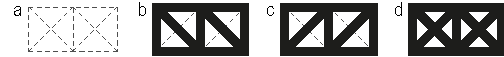
\includegraphics[width=\textwidth]{chapters/metamaterial-mechanisms-FIG/3-basic-grid-structure.pdf}
    \caption[Short figure name.]{(a) The basic grid structure allows reinforcing rigid member cells (b-c) with one diagonal or (d) two diagonals.
    \label{fig:3-basic-grid-structure}}
\end{figure}

While we will focus our discussion on only two types of cells, namely stiff member cells and shearable hinge cells, our research can be combined with any other system of metamaterials already done as long as they are on a cube grid. Just to pick one example, we can make cells soft or hard \cite{Chu2008a} by weakening their beams so as to allow the cells to compress more easily, or reinforcing their beams to make the cells stiffer (Figure \ref{fig:4-cells-increasing-stiffness}). 

\begin{figure} [h]
    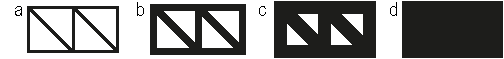
\includegraphics[width=\textwidth]{chapters/metamaterial-mechanisms-FIG/4-cells-increasing-stiffness.pdf}
    \caption[Short figure name.]{Member cells of increasing stiffness.
    \label{fig:4-cells-increasing-stiffness}}
\end{figure}


\subsection{Hinges}

We can create a (naïve) hinge by connecting two cells diagonally as shown in Figure \ref{fig:5-hinge-array}a. Here the material connecting the two cell blocks forms a thin flexible hinge made from the same material as the two rigid members it connects. As common for this type of contraption, we will refer to it as a living hinge.

\begin{figure} [h]
    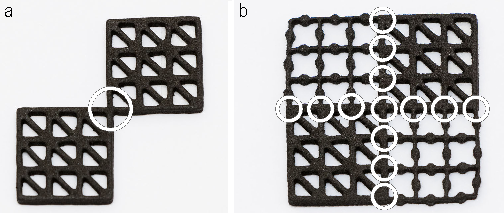
\includegraphics[width=\textwidth]{chapters/metamaterial-mechanisms-FIG/5-hinge-array.pdf}
    \caption[Short figure name.]{(a) A naïve living hinge, (b) reinforced with two arrays of hinges. To showcase the deformation, we laser cut these structures from rubber foam.
    \label{fig:5-hinge-array}}
\end{figure}

Next we add reinforcement to the hinge. Metamaterial cells can, at least in theory, be arbitrarily small—the hinge connecting two cells can thus arbitrarily thin, making mechanisms based on such naïve living hinges fragile, i.e., pulling them apart with very little force will rip them off.

We address the issue by extending the living hinge into an array of living hinges, as illustrated by Figure \ref{fig:5-hinge-array}b. We call them hinge arrays. Figure \ref{fig:6-simple-hinge-rotation} shows that the array flexes in concert with the main living hinge. The hinge array on the inside of the rotation complies by compressing in a shearing motion; the hinge array on the outside complies by stretching in a shearing motion. All hinges together perform a rotation around the original living hinge.

\begin{figure} [h]
    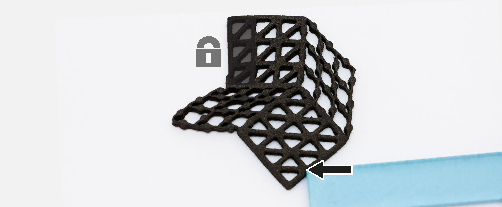
\includegraphics[width=\textwidth]{chapters/metamaterial-mechanisms-FIG/6-simple-hinge-rotation.pdf}
    \caption[Short figure name.]{The reinforced hinge in action. Note how the hinge array deforms as one while the rigid members remain undeformed. (Cells with gray tinted backgrounds are anchored to the ground, as indicated by the lock symbol. We are pushing in the direction of the arrow using the blue rod).
    \label{fig:6-simple-hinge-rotation}}
\end{figure}

However, when this reinforced hinge is stretched as shown in Figure \ref{fig:7-hinge-tear}a, its hinge arrays evade the tension by shearing. As a result, all tension rests on the central living hinge, causing it to break. As shown in Figure \ref{fig:7-hinge-tear}b, we address this by adding a border of rigid cells to the hinge arrays. These borders force all living hinges to follow the motion of the central living hinge, thereby support the main hinge by assuming part of the load, which distributes the tension across all the hinges.

Tensile strength increases linearly with the diagonal of the hinge array, because tension applies to the shortest path of hinges to tear in order to separate the two members. The tensile strength of the hinge array in Figure \ref{fig:7-hinge-tear}, for example, is $7\times$ larger than of a single hinge.

\begin{figure} [h]
    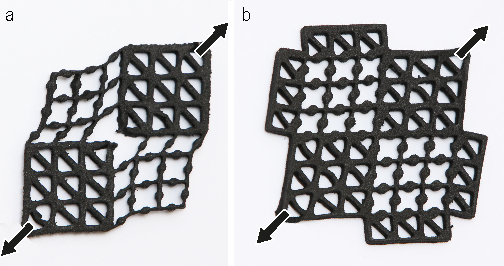
\includegraphics[width=\textwidth]{chapters/metamaterial-mechanisms-FIG/7-hinge-tear.pdf}
    \caption[Short figure name.]{(a) When this hinge array is stretched as shown, the central hinge breaks. (b) We address this by adding borders of rigid cells; they help distribute the tension more evenly. 
    \label{fig:7-hinge-tear}}
\end{figure}

Figure \ref{fig:8-simulation-tear-and-rotate} shows the resulting stress distribution after reinforcement (simulated using Autodesk Fusion 360; light colors indicate regions of high mechanical stress).

Hinge arrays also allow tuning the bending stiffness of a hinge, e.g., to make sure the door latch in Figure \ref{fig:1 metanism-door latch} offers appropriate resistance when pushed down, as well as sufficient force to push the handle back up. Bending stiffness increases proportional to the surface of the hinge array, i.e., $(width+1) \times (height+1)$, as all individual hinges need to be bent. The hinge array in Figure \ref{fig:7-hinge-tear}, for example, uses 2 hinge arrays of $(3+1) \times (3+1) = 32$ hinges, thus it takes 32 times more force to bend it than the single hinge in the center.

\begin{figure} [h]
    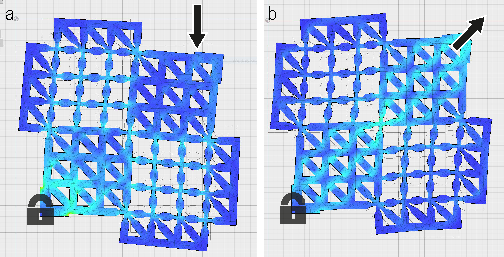
\includegraphics[width=\textwidth]{chapters/metamaterial-mechanisms-FIG/8-simulation-tear-and-rotate.pdf}
    \caption[Short figure name.]{Resulting stress distribution on (a) rotation and (b) tension after reinforcement.
    \label{fig:8-simulation-tear-and-rotate}}
\end{figure}


\subsection{Four-bars implement parallel motion}

In Figure \ref{fig:9-metamaterial-four-bar}, we use the concept of rigid members connected by hinge arrays to construct a shearing frame of four links, also known as \textit{four-bars}. Four-bars consist of four members attached to the \textit{opposite} sides of a hinge array (unlike the reinforced hinge, which consists of two members attached to \textit{adjacent} sides of a hinge array). It then contains the two opposing members to parallel motion. Note how the rigid member that is pushed to the left in Figure \ref{fig:9-metamaterial-four-bar}b rotates, while the top member moves in parallel with the rigid area underneath it.

\begin{figure} [h]
    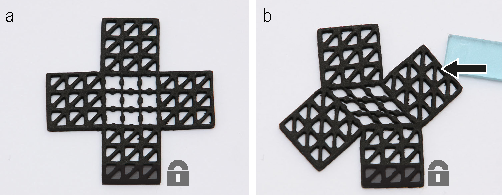
\includegraphics[width=\textwidth]{chapters/metamaterial-mechanisms-FIG/9-metamaterial-four-bar.pdf}
    \caption[Short figure name.]{A metamaterial four-bar. 
    \label{fig:9-metamaterial-four-bar}}
\end{figure}

In Figure \ref{fig:10-pliers-ninjaflex} we exploit this property of the four-bar in order to create a functional pair of pliers. The hinge array in the center acts as a four-bar that connects the right handle with the left bracket \textit{and} the left handle with the right bracket, yet allows the two sides to move with respect to each other---somewhat similar to how the axle in a traditional pair of scissors allows the two handle and blade elements to move with respect to each other.

\begin{figure} [h]
    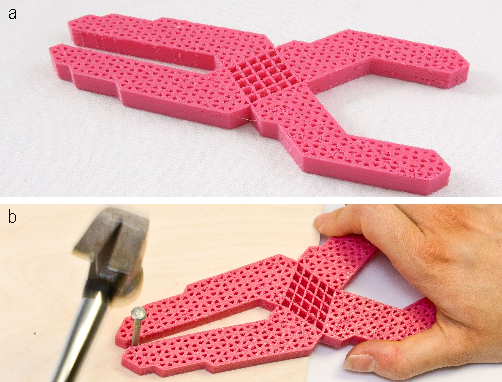
\includegraphics[width=\textwidth]{chapters/metamaterial-mechanisms-FIG/10-pliers-ninjaflex.pdf}
    \caption[Short figure name.]{(a) This pair of pliers is based on a single metamaterial four-bar. (b) When the user applies a force to the handles, the hinge array in the center transmits this force to the brackets, and the pliers close. 
    \label{fig:10-pliers-ninjaflex}}
\end{figure}


\subsection{Cascades of hinge arrays}

We chain multiple four-bars to create a scissors mechanism, which is a linkage that arranges links in a criss-cross pattern and is used. Figure \ref{fig:11-pantograph} shows how we implement a pantograph by chaining multiple metamaterial four-bars. The pantograph holds two pencils. While one pencil is moved by the user to draw, the second pencil moves along and replicates the user’s drawing.
 
\begin{figure} [h]  
    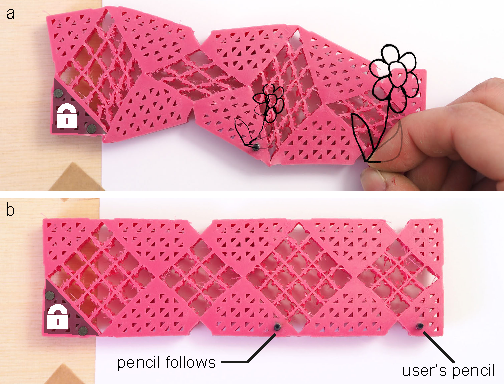
\includegraphics[width=\textwidth]{chapters/metamaterial-mechanisms-FIG/11-pantograph.pdf}
    \caption[Short figure name.]{The user draws a flower using (a) our metamaterial pantograph, which (b) replicates the flower as the user is drawing. 
    \label{fig:11-pantograph}}
\end{figure}


\section{The key: The shear cell}
\label{section:shear-cell}

So far, we only introduced the rigid cell. However, without explicitly mentioning it, the previous section introduced a second type of cell: a cell designed to shear. Unlike the rigid cell, this \textit{shear cell} is designed to deform when a force is applied, more specifically to \textit{shear} (Figure \ref{fig:12-shear-cell-deformation}). 

\begin{figure} [h]  
    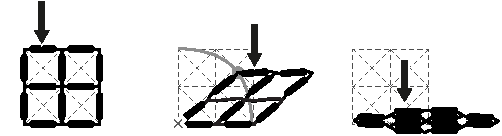
\includegraphics[width=\textwidth]{chapters/metamaterial-mechanisms-FIG/12-shear-cell-deformation.pdf}
    \caption[Short figure name.]{When a shear cell in this $2 \times 2$ block is subject to compression forces, it complies by shearing on a circular trajectory until its members are packed tightly.
    \label{fig:12-shear-cell-deformation}}
\end{figure}

As illustrated by Figure \ref{fig:12-shear-cell-deformation}, shear cells compress when a force is applied. The cell itself consists of miniature members and miniature living hinges---similar to the macroscopic structures we build from them. When a force is applied, the hinges start to bend, while the members largely maintain their shape (increasing the thickness of a beam results in a cubed increase in stiffness). The shear cell resists the external force based on the springiness of its hinges, until eventually the members touch and the resulting tightly packed block of cells is not compressible anymore apart from the compressibility of the material itself.

Since shear cells are based on an unit cell of our grid, they are always oriented along the cardinal directions. To allow handling forces and shearing along additional orientations, we introduce rotated hinges. As illustrated by Figure \ref{fig:13-diamond-cell-deformation}, we obtain a rotated design by combining groups of $2 \times 2$ cells, each of which contains (only) a diagonal. 

\begin{figure} [h]  
    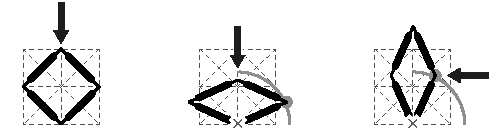
\includegraphics[width=\textwidth]{chapters/metamaterial-mechanisms-FIG/13-diamond-cell-deformation.pdf}
    \caption[Short figure name.]{The rotated shear cell.
    \label{fig:13-diamond-cell-deformation}}
\end{figure}

Combining regular and rotated hinges allows us to engineer additional mechanisms, such as the leg pair of a Jansen walker mechanism that is shown in Figure \ref{fig:14-jansen-walker}. Each leg consists of 6 hinges that make up the organic walking motion when the center is actuated on a circular path using a crank. One hinge per leg, however, needs to be constrained so as to only rotate, not translate. We implement this by adding a layer of two metamaterial hinges for the two legs that are connected to stay at constant distance but decoupled to move independently from each other. 

\begin{figure} [!h]
    \centering
    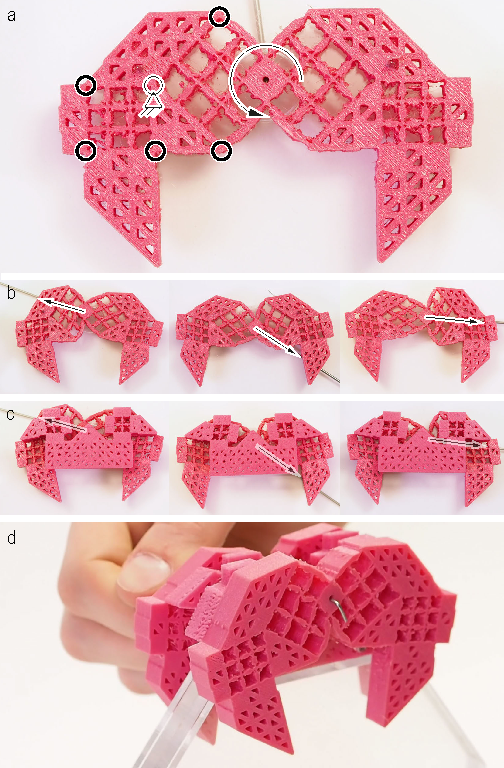
\includegraphics[width=0.83\textwidth]{chapters/metamaterial-mechanisms-FIG/14-jansen-walker.pdf}
    \caption[Short figure name.]{(a) Each leg of the Jansen walker has 6 hinges. (b) As the center is actuated by a crank, the legs deform in a walking motion. (c) We constrain two hinges to rotate, but not translate, using a layer of hinges. (d) The complete walker.
    \label{fig:14-jansen-walker}}
\end{figure}

Finally, we have created a third type of shear cell by leaving out one of the Cartesian members. It is shown in Figure \ref{fig:15-z-cell-deformation} and we refer to it as \textit{z-cell.}

\begin{figure} [!h]  
    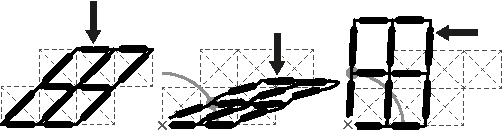
\includegraphics[width=\textwidth]{chapters/metamaterial-mechanisms-FIG/15-z-cell-deformation.pdf}
    \caption[Short figure name.]{"z-cells" shear on a larger circular path than regular shear cells, which is also rotated by 45°. 
    \label{fig:15-z-cell-deformation}}
\end{figure}

Z-cells are very similar to regular shear cells, except that they are “pre-sheared”, which results in three differences: (1) they have an asymmetric shearing behavior (range of 135° vs. 45°), (2) they expand as they shear against their pre-sheared direction, and (3) compress in the other direction.

Figure \ref{fig:16-switch} shows a switch based on z-cells. The button stays parallel while going down to hit the contact point reliably. A similar switch implemented from only soft and hard cells requires making very thin beams to allow the switch to deform. However, this does not implement a well-defined directional movement and closing at the contact point is not ensured.

\begin{figure} [h]
    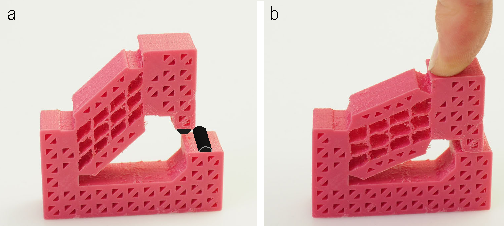
\includegraphics[width=\textwidth]{chapters/metamaterial-mechanisms-FIG/16-switch.pdf}
    \caption[Short figure name.]{(a) This switch is designed based on z-cells, which allow it to compress in a controlled motion and (b) close reliably at the black contact point. 
    \label{fig:16-switch}}
\end{figure}


\subsection{Padding}

Metamaterial mechanisms enable directional movement of regions of material, i.e., they occupy space when they are in their deformed state that was not occupied in their undeformed state. Most of our examples---the pliers, the walker, or the pantograph---are self-contained and can deform independently. However, the door latch is not self-contained but embedded in a rigid door. This requires appropriate clearance for the respective region to move into. 

We surround the door latch shown in Figure \ref{fig:17-padding-movement} with what we call padding areas. Padding areas consist of cells that are not intended to transmit any forces, but rather to receive the forces exerted by the main mechanism. The padding serves two purposes here: (1) to connect the movable door latch with the rigid door and (2) to increase its stability, i.e., to prevent the mechanism from buckling out of plane and add support against operation in unintended directions. In case the handle is pushed up, the z-cells above the latch prevent the latch from moving outward (to the right).

\begin{figure} [!h]
    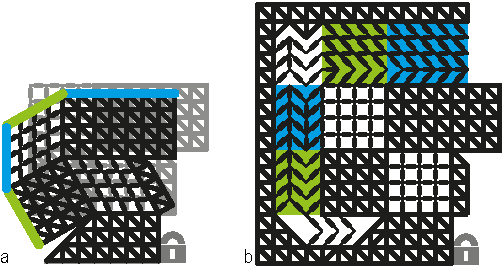
\includegraphics[width=\textwidth]{chapters/metamaterial-mechanisms-FIG/17-padding-movement.pdf}
    \caption[Short figure name.]{(a) When the door latch deforms, the edges labeled in blue remain parallel, while the green edges rotate. (b) Consequently, we reinforce the green regions using padding cells that allow for translation and rotation deformation, while we reinforce the blue regions to only allow for translation. 
    \label{fig:17-padding-movement}}
\end{figure}

Figure \ref{fig:17-padding-movement}a shows that after the door latch mechanism is deformed we see two types of transformations on the outside edges: (1) a parallel movement that is indicated by the blue line and (2) a rotational movement of the edge indicated by the green line. Additionally, all the edges undergo a vertical and horizontal translation. For all outside edges we need to allow translation and for some we need to additionally allow rotation. Therefore, the latch mechanism in Figure \ref{fig:17-padding-movement}b uses two types of padding cells, chosen to allow for the intended movement, yet to suppress other types of movement.

\paragraph{Z-cell padding absorbs parallel movement,} like the movement of the latch. Z-cell padding allows a member on one side to translate in 2D with respect to a member on the other side and keeps the two members parallel. Since z-cells shear on a circular path that is rotated by 45°, they allow for a vertical extension of $\sqrt{2}-1$ cells and a horizontal displacement of 1 cell. We simply stack enough layers of z-cells to compensate for the downward and inward movement of the latch.

Note that we added one row of z-cells that is flipped. Figure \ref{fig:18-padding-trajectories}a shows that this additional row is necessary since the shear cells underneath the latch and the z-cells above the latch travel on opposing circular trajectories and cannot pass each other. The flipped row of z-cells however moves upwards (Figure \ref{fig:18-padding-trajectories}b) and gives space for the lower row of z-cells to pass and thus the latch to move.

\begin{figure} [h]  
    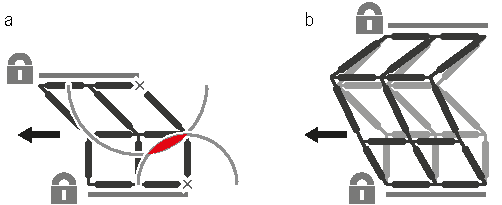
\includegraphics[width=\textwidth]{chapters/metamaterial-mechanisms-FIG/18-padding-trajectories.pdf}
    \caption[Short figure name.]{(a) The shear cells cannot pass each other (red area), (b) therefore we add a flipped row of z-cells that compress and give space for the other shearing cells to move.
    \label{fig:18-padding-trajectories}}
\end{figure}

\paragraph{V-cell padding absorbs rotation.} V-cells are similar to the flipped z-cell group, but they additionally allow two opposing members to rotate, as shown in Figure \ref{fig:19-v-cells}. We add this degree of freedom by removing the vertical beam from the z-cells. We use v-cells in combination with z-cells on the rotating edges illustrated by Figure \ref{fig:17-padding-movement}b. 

\begin{figure} [h]  
    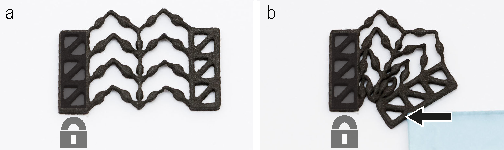
\includegraphics[width=\textwidth]{chapters/metamaterial-mechanisms-FIG/19-v-cells.pdf}
    \caption[Short figure name.]{V-cells allow for rotation, as well as for compression and extension.
    \label{fig:19-v-cells}}
\end{figure}


\section{Hierarchy of metamaterial mechanisms}

In this section, we presented the main elements of metamaterial mechanisms. These elements form the following five-level hierarchy.

\begin{enumerate}
    \item \textit{Cells} are the lowest-level element of metamaterial mechanisms and perform an elementary mechanical function. We presented shear cells, which implement four-bars on a cell level, as well as z-cells.
    \item \textit{Compound cells} still perform an elementary function, yet are implemented using multiple physical cells, such as the rotated shear cell or the v-cell.
    \item \textit{Basic mechanisms} are created by repeating cells, in particular the reinforced hinge mechanism and the four-bar mechanism.
    \item \textit{Compound mechanisms} consist of multiple basic mechanisms, such as the scissors mechanism implemented in the pantograph.
    \item \textit{Machines} perform a mechanical function and consist of one or more basic or compound mechanisms, such as the door latch (Figure \ref{fig:1 metanism-door latch} and Figure \ref{fig:17-padding-movement}), the pliers (Figure \ref{fig:10-pliers-ninjaflex}), the Jansen walker (Figure \ref{fig:14-jansen-walker}).
    
\end{enumerate}


% \section{Metamaterial Mechanisms Editor}

% To allow users to design, fabricate, and test metamaterials containing mechanisms we implemented the specialized editor shown in Figure \ref{fig:20-editor-ui}. 

% \begin{figure} [h]  
%     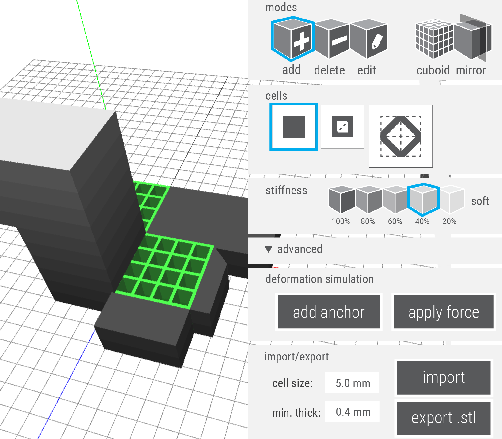
\includegraphics[width=\textwidth]{chapters/metamaterial-mechanisms-FIG/20-editor-ui.pdf}
%     \caption[Short figure name.]{Our editor allows users to edit and simulate the deformation of metamaterial mechanisms interactively. 
%     \label{fig:20-editor-ui}}
% \end{figure}

% The main intent behind it is not only to make the editing process more efficient than the more traditional script-based editing, but also to provide users with an overview of their design, encouraging design by trial-and-error. 

% Our editor is based on interaction techniques known from voxel editors (such as \textcolor{cyan}{[35]}). However, in addition our software also offers specific supports for creating mechanisms, such as tools for drawing hinge arrays, etc. In order to allow users to validate their designs, the editor also allows them to apply forces and see how the object deforms in order to then refine their design directly inside the editor, before exporting to the 3D printer.


% \subsection{Walkthrough}

% Figure \ref{fig:21-editor-walkthrough} illustrates how we created the door handle.

% (a) We start by creating a block of rigid cells using the \textit{add brush} (we can remove cells using the \textit{delete brush}). Here we use the tool in \textit{cuboid mode}, which allows us to draw a filled rectangular region at once by just drawing the diagonal. (b) By adding another two cuboids on top, we create the handle.

% (c) We select the \textit{shear brush}. Still in cuboid mode, we paint the central hinge array using a single drag interaction, which causes rigid cells to turn into shear cells. Even though the block of material we painted on is two cells high, the shear brush paints cells all the way through---as we can tell from the sidewall now being all green. This is one of the features of this brush: since shear cells backed by rigid cells would still be rigid, thus have no effect, the shear brush always cuts shear cells through the entire object. 

% \begin{figure} [h]  
%     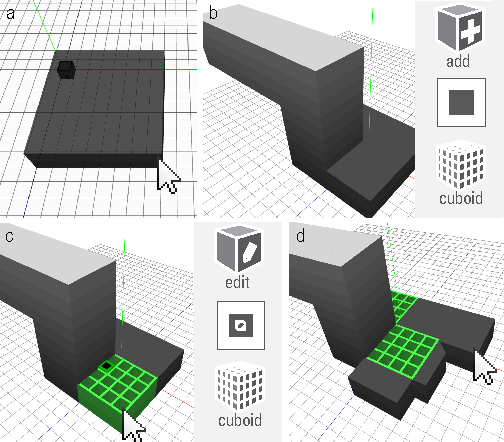
\includegraphics[width=\textwidth]{chapters/metamaterial-mechanisms-FIG/21-editor-walkthrough.pdf}
%     \caption[Short figure name.]{Walkthrough of the creating door latch mechanism. The UI elements on the right show the active tools for the respective interaction steps.
%     \label{fig:21-editor-walkthrough}}
% \end{figure}

% We now verify our design directly from within the editor, as illustrated by Figure \ref{fig:22-simulation-walkthrough}. (a) We select the anchor tool and use it to place a few anchor points at the bottom, indicating that the door latch is here rigidly connected to the doorframe. (b) Now we use the force tool to apply a force to the door handle. We attach a force arrow to one of the handle’s cell vertices. As we are building up the force by dragging the force tool the system already responds by showing the resulting deformation of our door latch. 

% \begin{figure} [h]  
%     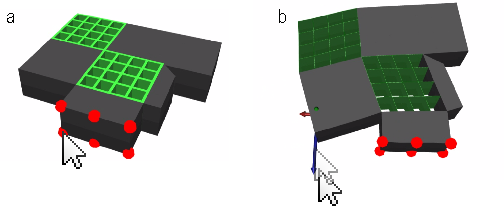
\includegraphics[width=\textwidth]{chapters/metamaterial-mechanisms-FIG/22-simulation-walkthrough.pdf}
%     \caption[Short figure name.]{To simulate the deformation in real-time in the editor, (a) users set anchor points and (b) adjust forces using the force tool. 
%     \label{fig:22-simulation-walkthrough}}
% \end{figure}


% \subsection{Multiple dimensions}

% While the door latch mechanism actuates in only two dimensions, our editor also supports placing mechanisms in 3 dimensions. The latch mechanism shown in Figure \ref{fig:23-3D-object}, for example, combines a horizontal hinge array (blue) and a vertical hinge array (green) in order to create a mechanism that users operate by pressing down, sliding over, and releasing. 

% Our editor color-codes mechanisms automatically according to their orientation in space. This is intended to provide users with a fast overview of the main dimensions of action in their devices and to help recognize hinge arrays from odd viewing angles. In the latch example, green denotes ``shearing on the x/z plane" and blue stands for ``shearing on the x/y plane". Analogously, red stands for ``shearing on the y/z plane".

% \begin{figure} [h]  
%     \includegraphics[width=\textwidth]{chapters/metamaterial-mechanisms-FIG/23-3D-object.pdf}
%     \caption[Short figure name.]{This latch requires the ability to shear on two planes, i.e., on the x/z plane denoted in green, and on the on x/y plane indicated in blue.
%     \label{fig:23-3D-object}}
% \end{figure}

% Note that hinge arrays can overlap. In this case, cells at the intersection bear the combination of all holes. These cells are rendered as the additive mixture of the involved colors, such as yellow, for cells at the intersection between green and red.


% \subsection{Integration with other metamaterial systems}

% The shear cell is the main element that enables metamaterial mechanisms. However, to allow for the integration with metamaterials by other researchers, the editor can be extended to allow for other cell types. 

% In order to allow users to explore their own cell types, we offer the advanced panel shown in Figure \ref{fig:24-advanced-cell-builder}. Users compose cells from individual edges by selecting the respective edges. The editor automatically adds all custom cells used in the current model to the cells panel for quick reuse. 

% \begin{figure} [h]  
%     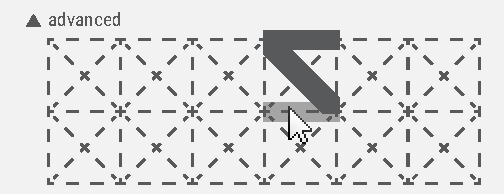
\includegraphics[width=\textwidth]{chapters/metamaterial-mechanisms-FIG/24-advanced-cell-builder.pdf}
%     \caption[Short figure name.]{Users compose custom cells by adding individual edges in the ``advanced" panel.
%     \label{fig:24-advanced-cell-builder}}
% \end{figure}

% Furthermore, users can also create and store groups of cells, for example to create auxetic materials \textcolor{cyan}{[6, 18]}, as shown in Figure \ref{fig:25-advanced-cell-groups}. Since metamaterial mechanisms adhere to the standard structure of 3D cell grids that is common for metamaterials, they integrate with earlier research \textcolor{cyan}{[24, 30]}.

% \begin{figure} [h]  
%     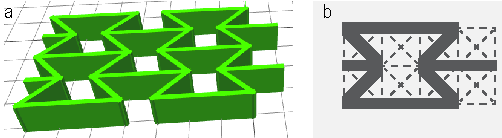
\includegraphics[width=\textwidth]{chapters/metamaterial-mechanisms-FIG/25-advanced-cell-groups.pdf}
%     \caption[Short figure name.]{Users add groups of cells, here they create an auxetic material from a $4 \times 2$ group of cells.
%     \label{fig:25-advanced-cell-groups}}
% \end{figure}


% \section{System Implementation}
% \label{section:mechanisms-editor}

% In the following, we provide details on the internal processes implemented in our metamaterial mechanisms editor.

% \subsection{Import}

% Users can import mesh geometries directly into our editor. We voxelize the meshes using \textit{binvox}\footnote{\url{http://www.cs.princeton.edu/~min/binvox/}}  according to the cell size that the user defined. 

% \subsection{Editor}
% Our 3D editor is based on WebGL and uses three.js. Internally, the editor creates a dictionary of cells that can be accessed using their position on the grid. Each cell is defined by the 8 vertices making up its bounding box by and the edges that define how the vertices are connected. Note that not all 8 vertices need to be connected by edges. 

% All vertices lie on our uniform 3-dimensional grid. To generate the 3D cells' structures, i.e., to generate 3D beams from 1D edges, we apply an offset to the vertices’ positions on the GPU. Since WebGL does not offer geometry shaders, we use a vertex shader and pass the offset direction and the cell’s position with each vertex. The 8 vertices that form a beam are offset uniformly from the two edge vertices on the GPU. To pass additional information about the color and thickness of beams to the shader, we generate a texture where each pixel holds these data for one cell. The color maps directly and the thickness is encoded in the alpha component. In the shader, every vertex looks up its thickness in the texture and calculates the offsets for the new vertices that render a beam from an edge. This enables us to emulate a geometry shader in WebGL and perform all geometry processing on the GPU, which keeps the user experience of our editor smooth.

% \subsection{Simulation}
% For simulating the deformation of the user’s cell structure, we use the finite elements solver \textit{karamba}\footnote{\url{http://www.karamba3d.com/}}, which is a plugin-for Grasshopper/Rhinoceros. We implemented a custom C\#-Grasshopper-component that receives the mesh data (vertices and edges) and the data for the simulation (anchored vertices, force and vertex where the force applies) via a web socket connection. When the simulation is complete, a second custom component receives the transformed mesh vertices and sends them back to the editor. The vertices are kept in the same order within the array as they were received from the editor. We run the simulation on a separate machine to keep the editor running smoothly. 

% Maintaining the order of the vertices is important to enable geometry processing on the GPU. In the editor, we generate another texture and store the transformed vertices, where XYZ is mapped to RGB. The shader knows the vertex' undeformed position on the grid and looks up the deformed position in the texture.

% Depending on the size of the object that is simulated, solving for the deformation can lead to perceivable delays. To compensate for this, our editor interpolates the deformation while the response from the simulation is pending. To do so, we pass the last force where we received the transformation from the server, and the current force that was submitted to the simulation and interpolate the vertex transformation linearly.

% \subsection{Export}

% We generate an .stl file for the user that is ready to be 3D printed. Our export is based on OpenJSCAD. In this step, we refine the cell structure from the simplified editor view to our beams with stiff members and thin living hinges. For every edge that belongs to a shear cell, we create a beam with a thick part in the middle. Edges that are part of rigid cells are generated as simple straight beams. Finally, we use OpenJSCAD's built-in render engine, which we invoke directly from our 3D editor to perform the union operations and generate the .stl file.


\section{Editing metamaterial mechanisms}

To allow users to design, fabricate, and test metamaterials containing mechanisms we implemented the specialized editor shown in Figure \ref{fig:20-editor-ui}. 

\begin{figure} [h]
    \centering
    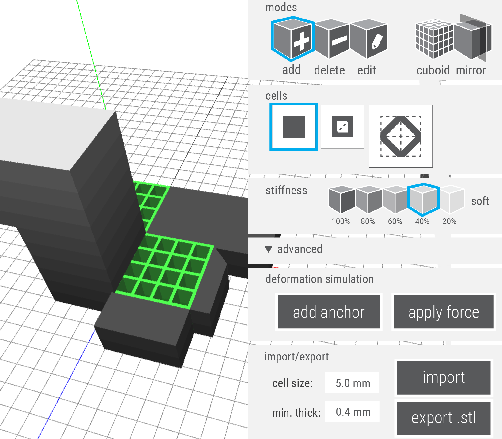
\includegraphics[width=0.9\textwidth]{chapters/metamaterial-mechanisms-FIG/20-editor-ui.pdf}
    \caption[Short figure name.]{Our editor allows users to edit and simulate the deformation of metamaterial mechanisms interactively. 
    \label{fig:20-editor-ui}}
\end{figure}

The main intent behind it is not only to make the editing process more efficient than the more traditional script-based editing, but also to provide users with an overview of their design, encouraging design by trial-and-error. 

Our editor is based on interaction techniques known from voxel editors (such  as \cite{VoxCAD2018}). However, in addition our software also offers specific supports for creating mechanisms, such as tools for drawing hinge arrays, etc. In order to allow users to validate their designs, the editor also allows them to apply forces and see how the object deforms in order to then refine their design directly inside the editor, before exporting to the 3D printer.

%\section{Encapsulating domain knowledge into the editor}

\subsection{User interaction}

Figure \ref{fig:21-editor-walkthrough} illustrates how users create the door handle example.

\begin{figure} [h]
    \centering
    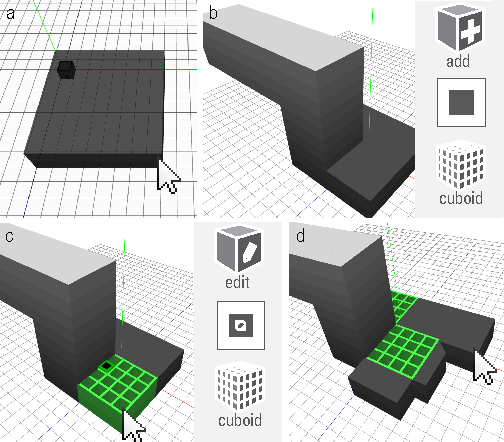
\includegraphics[width=0.85\textwidth]{chapters/metamaterial-mechanisms-FIG/21-editor-walkthrough.pdf}
    \caption[Short figure name.]{Walkthrough of the creating door latch mechanism. The UI elements on the right show the active tools for the respective interaction steps.
    \label{fig:21-editor-walkthrough}}
\end{figure}

(a) Users start by creating a block of rigid cells using the \textit{add brush}. They can remove cells using the \textit{delete brush}. Here, users utilize the tool in \textit{cuboid mode}, which allows them to draw a filled rectangular region at once by just drawing the diagonal. (b) By adding another two cuboids on top, users create the handle.

(c) Next, Users select the \textit{shear brush}. Still in cuboid mode, they paint the central hinge array using a single drag interaction, which causes rigid cells to turn into shear cells. Even though the block of material that users painted on is two cells high, the shear brush paints cells all the way through---as they can tell from the sidewall now being all green. This is one of the features of this brush: since shear cells backed by rigid cells would still be rigid, thus have no effect, the shear brush always cuts shear cells through the entire object. 


\subsection{Simulating deformation}
Users now verify their design directly from within the editor, as illustrated by Figure \ref{fig:22-simulation-walkthrough}. 

\begin{figure} [h]
    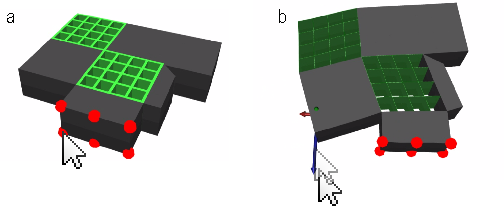
\includegraphics[width=\textwidth]{chapters/metamaterial-mechanisms-FIG/22-simulation-walkthrough.pdf}
    \caption[Short figure name.]{To simulate the deformation in real-time in the editor, (a) users set anchor points and (b) adjust forces using the force tool. 
    \label{fig:22-simulation-walkthrough}}
\end{figure}

(a) They select the anchor tool and use it to place a few anchor points at the bottom, indicating that the door latch is rigidly connected to the doorframe there. (b) Now, they use the force tool to apply a force to the door handle. Users attach a force arrow to one of the handle’s cell vertices. As users are building up the force by dragging the force tool the system already responds by showing the resulting deformation of our door latch. 

\subsection{Multiple dimensions}
While the door latch mechanism actuates in only two dimensions, our editor also supports placing mechanisms in 3 dimensions. The latch mechanism shown in Figure \ref{fig:23-3D-object}, for example, combines a horizontal hinge array (blue) and a vertical hinge array (green) in order to create a mechanism that users operate by pressing down, sliding over, and releasing. 

\begin{figure} [h]
    \includegraphics[width=\textwidth]{chapters/metamaterial-mechanisms-FIG/23-3D-object.pdf}
    \caption[Short figure name.]{This latch requires the ability to shear on two planes, i.e., on the x/z plane denoted in green, and on the on x/y plane indicated in blue.
    \label{fig:23-3D-object}}
\end{figure}

Our editor color-codes mechanisms automatically according to their orientation in space. This is intended to provide users with a fast overview of the main dimensions of action in their devices and to help recognize hinge arrays from odd viewing angles. In the latch example, green denotes ``shearing on the x/z plane" and blue stands for ``shearing on the x/y plane". Analogously, red stands for ``shearing on the y/z plane".

Note that hinge arrays can overlap. In this case, cells at the intersection bear the combination of all holes. These cells are rendered as the additive mixture of the involved colors, such as yellow, for cells at the intersection between green and red.


\subsection{Integrating other metamaterial systems}

The shear cell is the main element that enables metamaterial mechanisms. However, to allow for the integration with metamaterials by other researchers, the editor can be extended to allow for other cell types. 

In order to allow users to explore their own cell types, we offer the advanced panel shown in Figure \ref{fig:24-advanced-cell-builder}. Users compose cells from individual edges by selecting the respective edges. The editor automatically adds all custom cells used in the current model to the cells panel for quick reuse. 

\begin{figure} [h]
    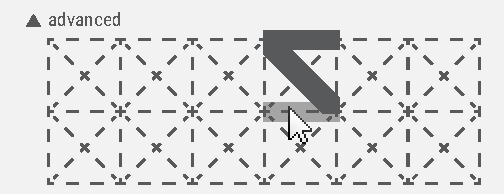
\includegraphics[width=\textwidth]{chapters/metamaterial-mechanisms-FIG/24-advanced-cell-builder.pdf}
    \caption[Short figure name.]{Users compose custom cells by adding individual edges in the ``advanced" panel.
    \label{fig:24-advanced-cell-builder}}
\end{figure}

Furthermore, users can also create and store groups of cells, for example to create auxetic materials \cite{Saxena2016}, as shown in Figure \ref{fig:25-advanced-cell-groups}. Since metamaterial mechanisms adhere to the standard structure of 3D cell grids that is common for metamaterials, they integrate with earlier research \cite{Panetta2015, Schumacher2015}.

\begin{figure} [h]
    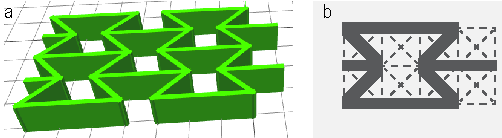
\includegraphics[width=\textwidth]{chapters/metamaterial-mechanisms-FIG/25-advanced-cell-groups.pdf}
    \caption[Short figure name.]{Users add groups of cells, here they create an auxetic material from a $4 \times 2$ group of cells.
    \label{fig:25-advanced-cell-groups}}
\end{figure}


\subsection{Implementation}
\label{section:mechanisms-editor}

In the following, we provide details on the internal processes implemented in our metamaterial mechanisms editor.

\subsubsection{Editor (.js)}
Our 3D editor is based on WebGL and uses three.js. Internally, the editor creates a dictionary of cells that can be accessed using their position on the grid. Each cell is defined by the 8 vertices making up its bounding box by and the edges that define how the vertices are connected. Note that not all 8 vertices need to be connected by edges. 

All vertices lie on our uniform 3-dimensional grid. To generate the 3D cells' structures, i.e., to generate 3D beams from 1D edges, we apply an offset to the vertices’ positions on the GPU. Since WebGL does not offer geometry shaders, we use a vertex shader and pass the offset direction and the cell’s position with each vertex. The 8 vertices that form a beam are offset uniformly from the two edge vertices on the GPU. To pass additional information about the color and thickness of beams to the shader, we generate a texture where each pixel holds these data for one cell. The color maps directly and the thickness is encoded in the alpha component. In the shader, every vertex looks up its thickness in the texture and calculates the offsets for the new vertices that render a beam from an edge. This enables us to emulate a geometry shader in WebGL and perform all geometry processing on the GPU, which keeps the user experience of our editor smooth.

\subsubsection{Simulation (C\#)}
For simulating the deformation of the user’s cell structure, we use the finite elements solver \textit{karamba}\footnote{\url{http://www.karamba3d.com/}} \cite{Preisinger2013}, which is a plugin-for Grasshopper/Rhinoceros. We implemented a custom C\#-Grasshopper-component that receives the mesh data (vertices and edges) and the data for the simulation (anchored vertices, force and vertex where the force applies) via a web socket connection. When the simulation is complete, a second custom component receives the transformed mesh vertices and sends them back to the editor. The vertices are kept in the same order within the array as they were received from the editor. We run the simulation on a separate machine to keep the editor running smoothly. 

Maintaining the order of the vertices is important to enable geometry processing on the GPU. In the editor, we generate another texture and store the transformed vertices, where XYZ is mapped to RGB. The shader knows the vertex' undeformed position on the grid and looks up the deformed position in the texture.

Depending on the size of the object that is simulated, solving for the deformation can lead to perceivable delays. To compensate for this, our editor interpolates the deformation while the response from the simulation is pending. To do so, we pass the last force where we received the transformation from the server, and the current force that was submitted to the simulation and interpolate the vertex transformation linearly.

\subsubsection{Import \& export}

Users can import mesh geometries directly into our editor. We load .stl meshes using the package 'stl-reader'\footnote{\url{https://www.npmjs.com/package/stl-reader}} and voxelize\footnote{\url{https://www.npmjs.com/package/voxelize}} them according to the cell size that the user defined. Once users are satisfied with their metamaterial, they can export their design as a 3D-printable .stl file. We use a constructive solid geometry (CSG) package\footnote{\url{https://www.npmjs.com/package/openjscad-csg}},
which we invoke directly from our 3D editor to perform the union operations and generate a triangulated .stl file.


\subsection{Software architecture}

We designed out software to be loosely coupled. As depicted in Figure \ref{fig:simple-software-architecture}, our editor communicates with the finite element analysis (FEA) tool via a web socket connection. This architecture allow the resource-intensive FEA calculations to be outsourced to a different computer (server) and to exchange the FEA component easily. 

\begin{figure} [h]
    \centering 
    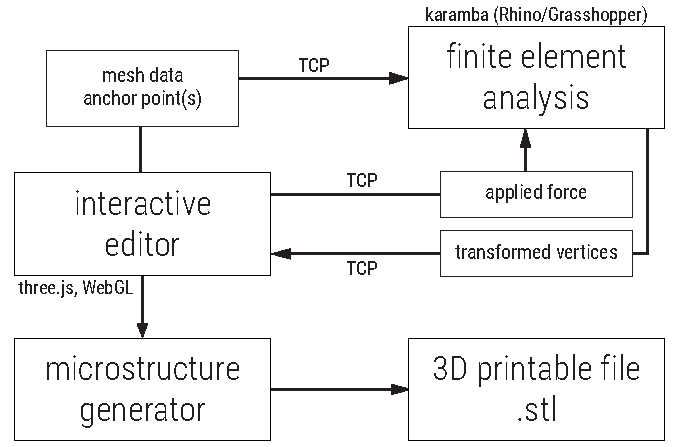
\includegraphics[width=0.85\textwidth]{chapters/software-FIG/simple-software-architecture.pdf}
    \caption[Short figure name.]{The software architecture or our metamaterial mechanism editor.
    \label{fig:simple-software-architecture}}
\end{figure}



\section{Discussion on material \& durability}

The ideal material for metamaterial mechanisms is (1) very elastic, i.e., goes back to its original shape without deforming permanently and (2) can withstand high forces without breaking. Spring steel fulfills these criteria well, yet is not possible to fabricate using today’s 3D printers. Among commonly available 3D printing materials, flexible materials (such as the TPU \textit{NinjaFlex} and \textit{SemiFlex}) fulfill these criteria well, more so than PLA and certain types of photo-curing resins (such as the \textit{spot-e} resin).

When we created 2D metamaterial mechanisms using our laser cutter, we obtained best results with rubber foam, more so than with ABS sheets and acrylic, which were not compliant enough. Our metamaterial mechanisms worked across fabrication techniques, since the functionality is determined by the cell structure. 

In our experience, material fatigue is not a problem, because we operate our metamaterial mechanisms, i.e., bend their living hinges, only to the point where they still fully return to their original shape (the material stays ``in the elastic region"). As an example, operating the NinjaFlex-printed Jansen walker shown in Figure \ref{fig:26-durability-test-jansen} about {\textasciitilde}5000 times (at {\textasciitilde}120 rpm) using a 300 W power drill, did not lead to any visible fatigue or damage in the metamaterial structure. 

\begin{figure} [h]  
    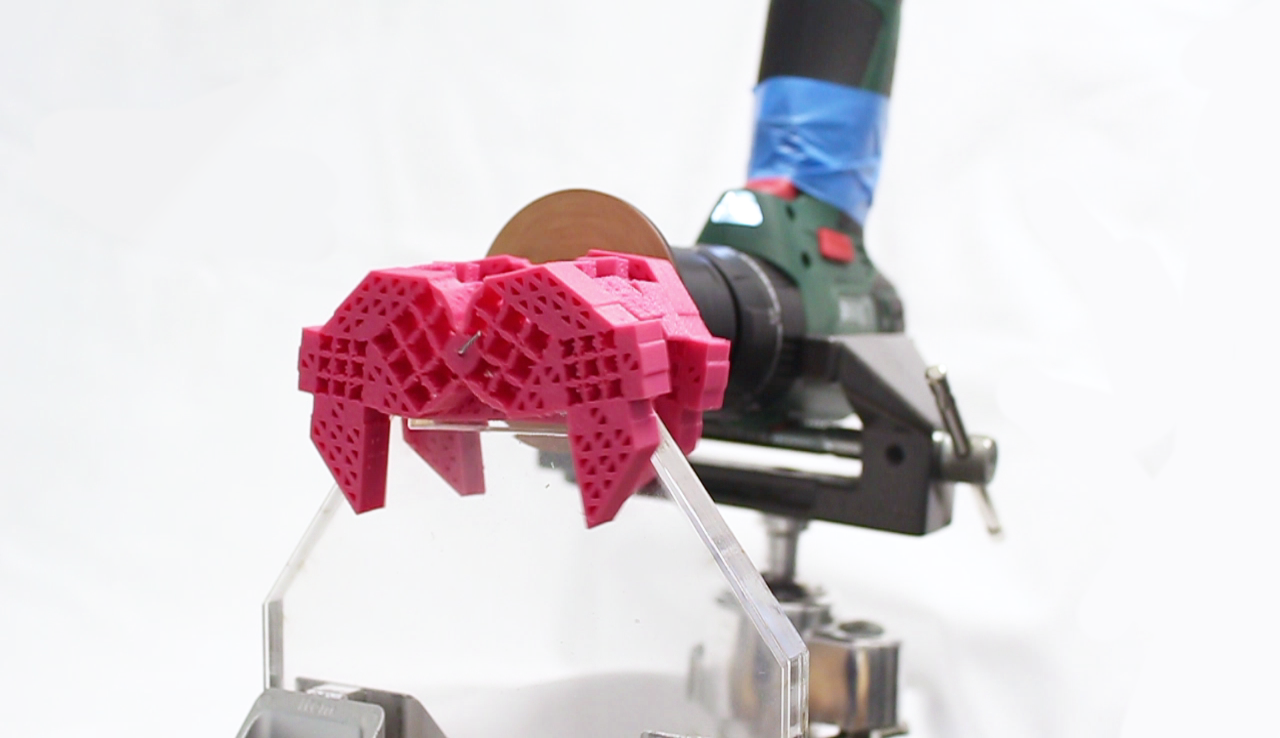
\includegraphics[width=\textwidth]{chapters/metamaterial-mechanisms-FIG/26-durability-test-jansen.png}
    \caption[Short figure name.]{We verified the durability of the Jansen walker by operating it {\textasciitilde}5000 times using a power drill.
    \label{fig:26-durability-test-jansen}}
\end{figure}

\section{Conclusions}
In this paper, we introduced metamaterial mechanisms. While metamaterials so far had been understood as materials, the main contribution of this paper is that we think of them as \textit{machines.}

On the most basic level, it was the shear cell that allowed us to implement this new perspective on metamaterials. The shear cell allowed us to redirect forces and thus to create basic mechanisms, compound mechanisms, and ultimately simple machines.

While our approach offers tangible benefits for users (e.g., it solves mechanical problems in a single part, thereby eliminates the need for assembly), we see the main promise of this work in that it allows us to achieve a deeper integration between the structural and the mechanical functions of materials.

% For future work, we plan to continue on this path by investigating how to integrate logical functions into material.

% Acknowledgements
% We thank David Lindlbauer for his insights and for printing many of our prototypes. We also thank Louis Kirsch, Moritz Hilscher, David Stangl, Arthur Silber, Friedrich Horschig and Noel Danz for their contribution to earlier versions of this work. 
